\section{The reserve trade-off}
\label{sec:reserve-tradeoff}

Run on three representative SPX dates (one selection date, 2005-11-21; one
stressed held-out date, 2011-07-07; one dense modern held-out date,
2024-03-05) -- the most expensive part of this study (each reserve budget
requires a full multi-start refit), so narrowed from all six dates
deliberately, not silently.

\paragraph{Setup.} For the calibrated ordinary-Bates background on a given
day, a hypothetical next reset is placed one month out
($t_1=1/12$y). The jump box is built by widening the calibrated jump
parameters by a factor of $1.5$ (Sec.~\texttt{config.JUMP\_BOX\_WIDEN\_FACTOR}),
and $[\theta_{\min},\theta_{\max}]=\theta_0\pm0.03$. Reserve budget
$r_1\in\{0,0.01,0.03,0.06\}$ is swept ($r_1=0$ is the degenerate/ordinary-Bates
case: no schedule can be built since \texttt{ReserveSchedule} requires
strictly positive reserve sizes).

\paragraph{(1) Fit cost of turning on the reserve, before recalibration --
LARGE, not small.} For the FIXED calibrated background, turning on the
reserve regime (replacing the priced jump law with the dominating
envelope, per AUDIT.md Sec.~8/10's cancellation identity) shifts prices at
EVERY expiry, not only those beyond $t_1$: mean relative price shift
\textbf{195--276\%} across the tested dates/budgets, and bid-ask coverage
collapses from the ordinary-Bates baseline (94--100\% on the two dates
where it is well-fit) to \textbf{0\%} immediately. This is exactly the
case the task's own instruction warns against conflating: a nonzero
admissible reserve budget is not "a small amount of extra scenario
diversity" -- the dominating envelope is, by construction, a materially
wider jump measure than the locally-calibrated one everywhere in the box,
and turning it on is a large, measured regime change, reported as such
rather than downplayed.

\paragraph{(2) Cost recovered by recalibration -- most, not all, and not
always.} The whole admissible model (chain $\kappa$, anchor width, Bates
background) is then refit UNDER the extended-Bates+reserve regime at the
same fixed budget. On 2005-11-21 and 2011-07-07, coverage recovers to
46--78\% (still below the 94--100\% ordinary-Bates baseline) and mean fit
error drops from $\sim$40 to $0.3$--$1.05$ (baseline $\sim$0.0--0.01) --
substantial, genuine, but incomplete recovery. On 2024-03-05 -- the date
where the ordinary-Bates baseline was ALREADY the weakest (20\% inside
bid-ask, Table~\ref{tab:main-comparison}) -- recalibration under the
reserve regime \textbf{fails to converge at every one of the three tested
budgets} (\texttt{ChainExtendedBatesCalibrationError}, both multi-start
attempts unsuccessful): a genuine solver failure, recorded as such, not
hidden or silently retried. Figure~\ref{fig:fit-vs-recalibration} shows the
recoverable dates directly.

\paragraph{Once established, subsequent resets are comparatively cheap.}
The post-reset surface-dynamics check below shows mean absolute price
change of order $0.0005$--$0.005$ for the most extreme admissible
upward/downward $\theta$ move -- one to two orders of magnitude smaller
than the cost of establishing the reserve regime itself (order
$0.03$--$0.07$). Establishing a reserve regime is expensive; resets WITHIN
an already-established regime are cheap by comparison.

\paragraph{Admissible $\theta$ movement and post-reset surface dynamics.}
For each budget, \texttt{admissible\_delta\_interval} reports the exact
upward/downward $\theta$ range a future reset could realise; applying the
two EXTREMES of that interval (not merely "a nonzero change exists")
reprices every evaluation contract beyond $t_1$ before/after, reported as
mean absolute price change in Table~\ref{tab:reserve-sweep}. Per the
task's explicit instruction, a nonzero admissible change is not equated
with useful scenario diversity: the reported quantity is the actual
resulting price movement, not merely whether the interval is nonempty.

\begin{table}[H]
\centering
\small
\begin{tabular}{llllllll}
\toprule
Date & $r_1$ & baseline (r=0) & shift & before recalib. & after recalib. & adm. $\Delta\theta$ & post-reset $|\Delta$price$|$ (up/down) \\
& & \%inside/err & (mean rel.) & \%inside/err & \%inside/err & interval & mean abs \\
\midrule
2005-11-21 & 0.01 & 100\%/0.00 & 195\% & 0\% / 39.70 & 62\% / 0.59 & [-0.030,0.010] & 0.0018 / 0.0049 \\
2005-11-21 & 0.03 &  & 211\% & 0\% / 44.27 & 46\% / 0.75 & [-0.030,0.030] & 0.0051 / 0.0045 \\
2005-11-21 & 0.06 &  & 237\% & 0\% / 50.84 & 50\% / 1.05 & [-0.030,0.030] & 0.0045 / 0.0041 \\
2011-07-07 & 0.01 & 94\%/0.01 & 259\% & 0\% / 39.74 & 78\% / 0.36 & [-0.030,0.010] & 0.0006 / 0.0018 \\
2011-07-07 & 0.03 &  & 265\% & 0\% / 40.84 & 73\% / 0.30 & [-0.030,0.030] & 0.0018 / 0.0018 \\
2011-07-07 & 0.06 &  & 273\% & 0\% / 42.47 & 71\% / 0.36 & [-0.030,0.030] & 0.0018 / 0.0018 \\
2024-03-05 & 0.01 & 20\%/1.43 & 273\% & 0\% / 600.66 & FAILED & -- & -- \\
2024-03-05 & 0.03 &  & 275\% & 0\% / 604.91 & FAILED & -- & -- \\
2024-03-05 & 0.06 &  & 276\% & 0\% / 611.23 & FAILED & -- & -- \\
\bottomrule
\end{tabular}

\caption{Reserve trade-off summary across the three representative dates and swept budgets.}
\label{tab:reserve-sweep}
\end{table}

\begin{figure}[H]
\centering
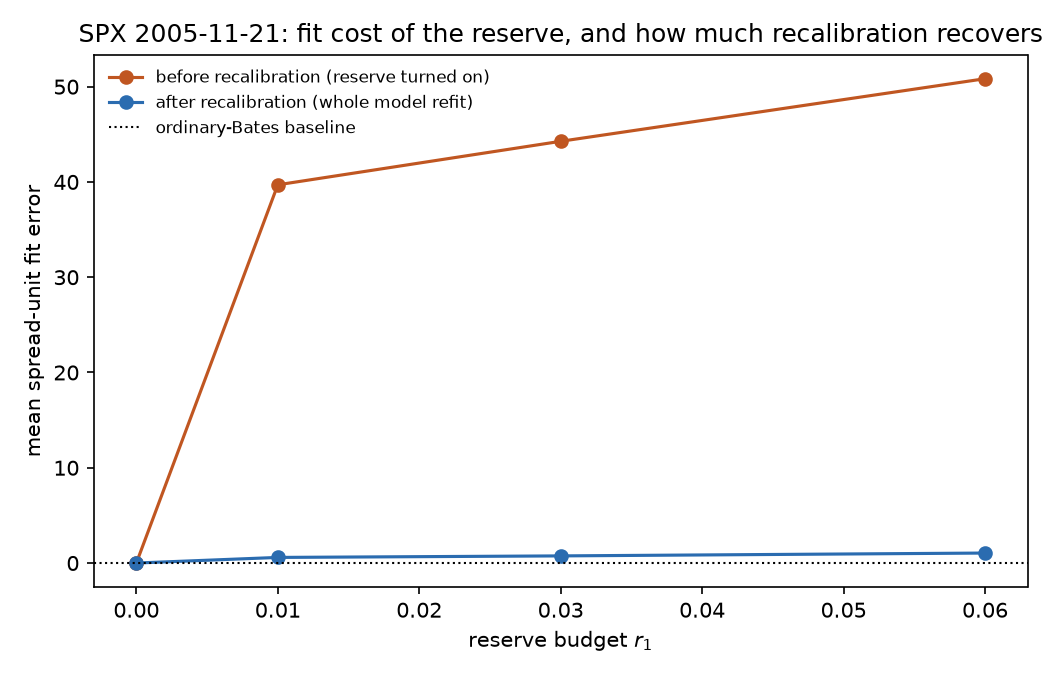
\includegraphics[width=0.85\textwidth]{figures/fit_vs_recalibration_freedom_SPX_2005-11-21.png}
\caption{Fit cost of the reserve before recalibration, and how much recalibration recovers, 2005-11-21.}
\label{fig:fit-vs-recalibration}
\end{figure}
